% !TEX encoding = UTF-8
% !TEX TS-program = pdflatex
% !TEX root = ../Tesi.tex
% !TEX spellcheck = en-EN

%************************************************
\chapter{Prologue}
\label{cap:prologue}
%************************************************

Particles in various forms - ranging from raw materials to food grains and pharmaceutical powders - 
play a major role in a variety of industries, including process industry and metallurgy. 
In his book, \citet{RefWorks:117} stated that "between 1 and 10\% of all the energy is used in 
comminution, i.e. the processes of crushing, grinding, milling, micronising". 
Many methods have been developed to study particles.
For instance, Discrete Element Methods (\acs{DEMs}), "a special class of numerical
schemes for simulating the behavior of discrete, interacting bodies", are widely used to 
simulate particle behaviour in these granular processes
(\citet{RefWorks:130}).\\ 
\begin{figure}[!htb]
\centering
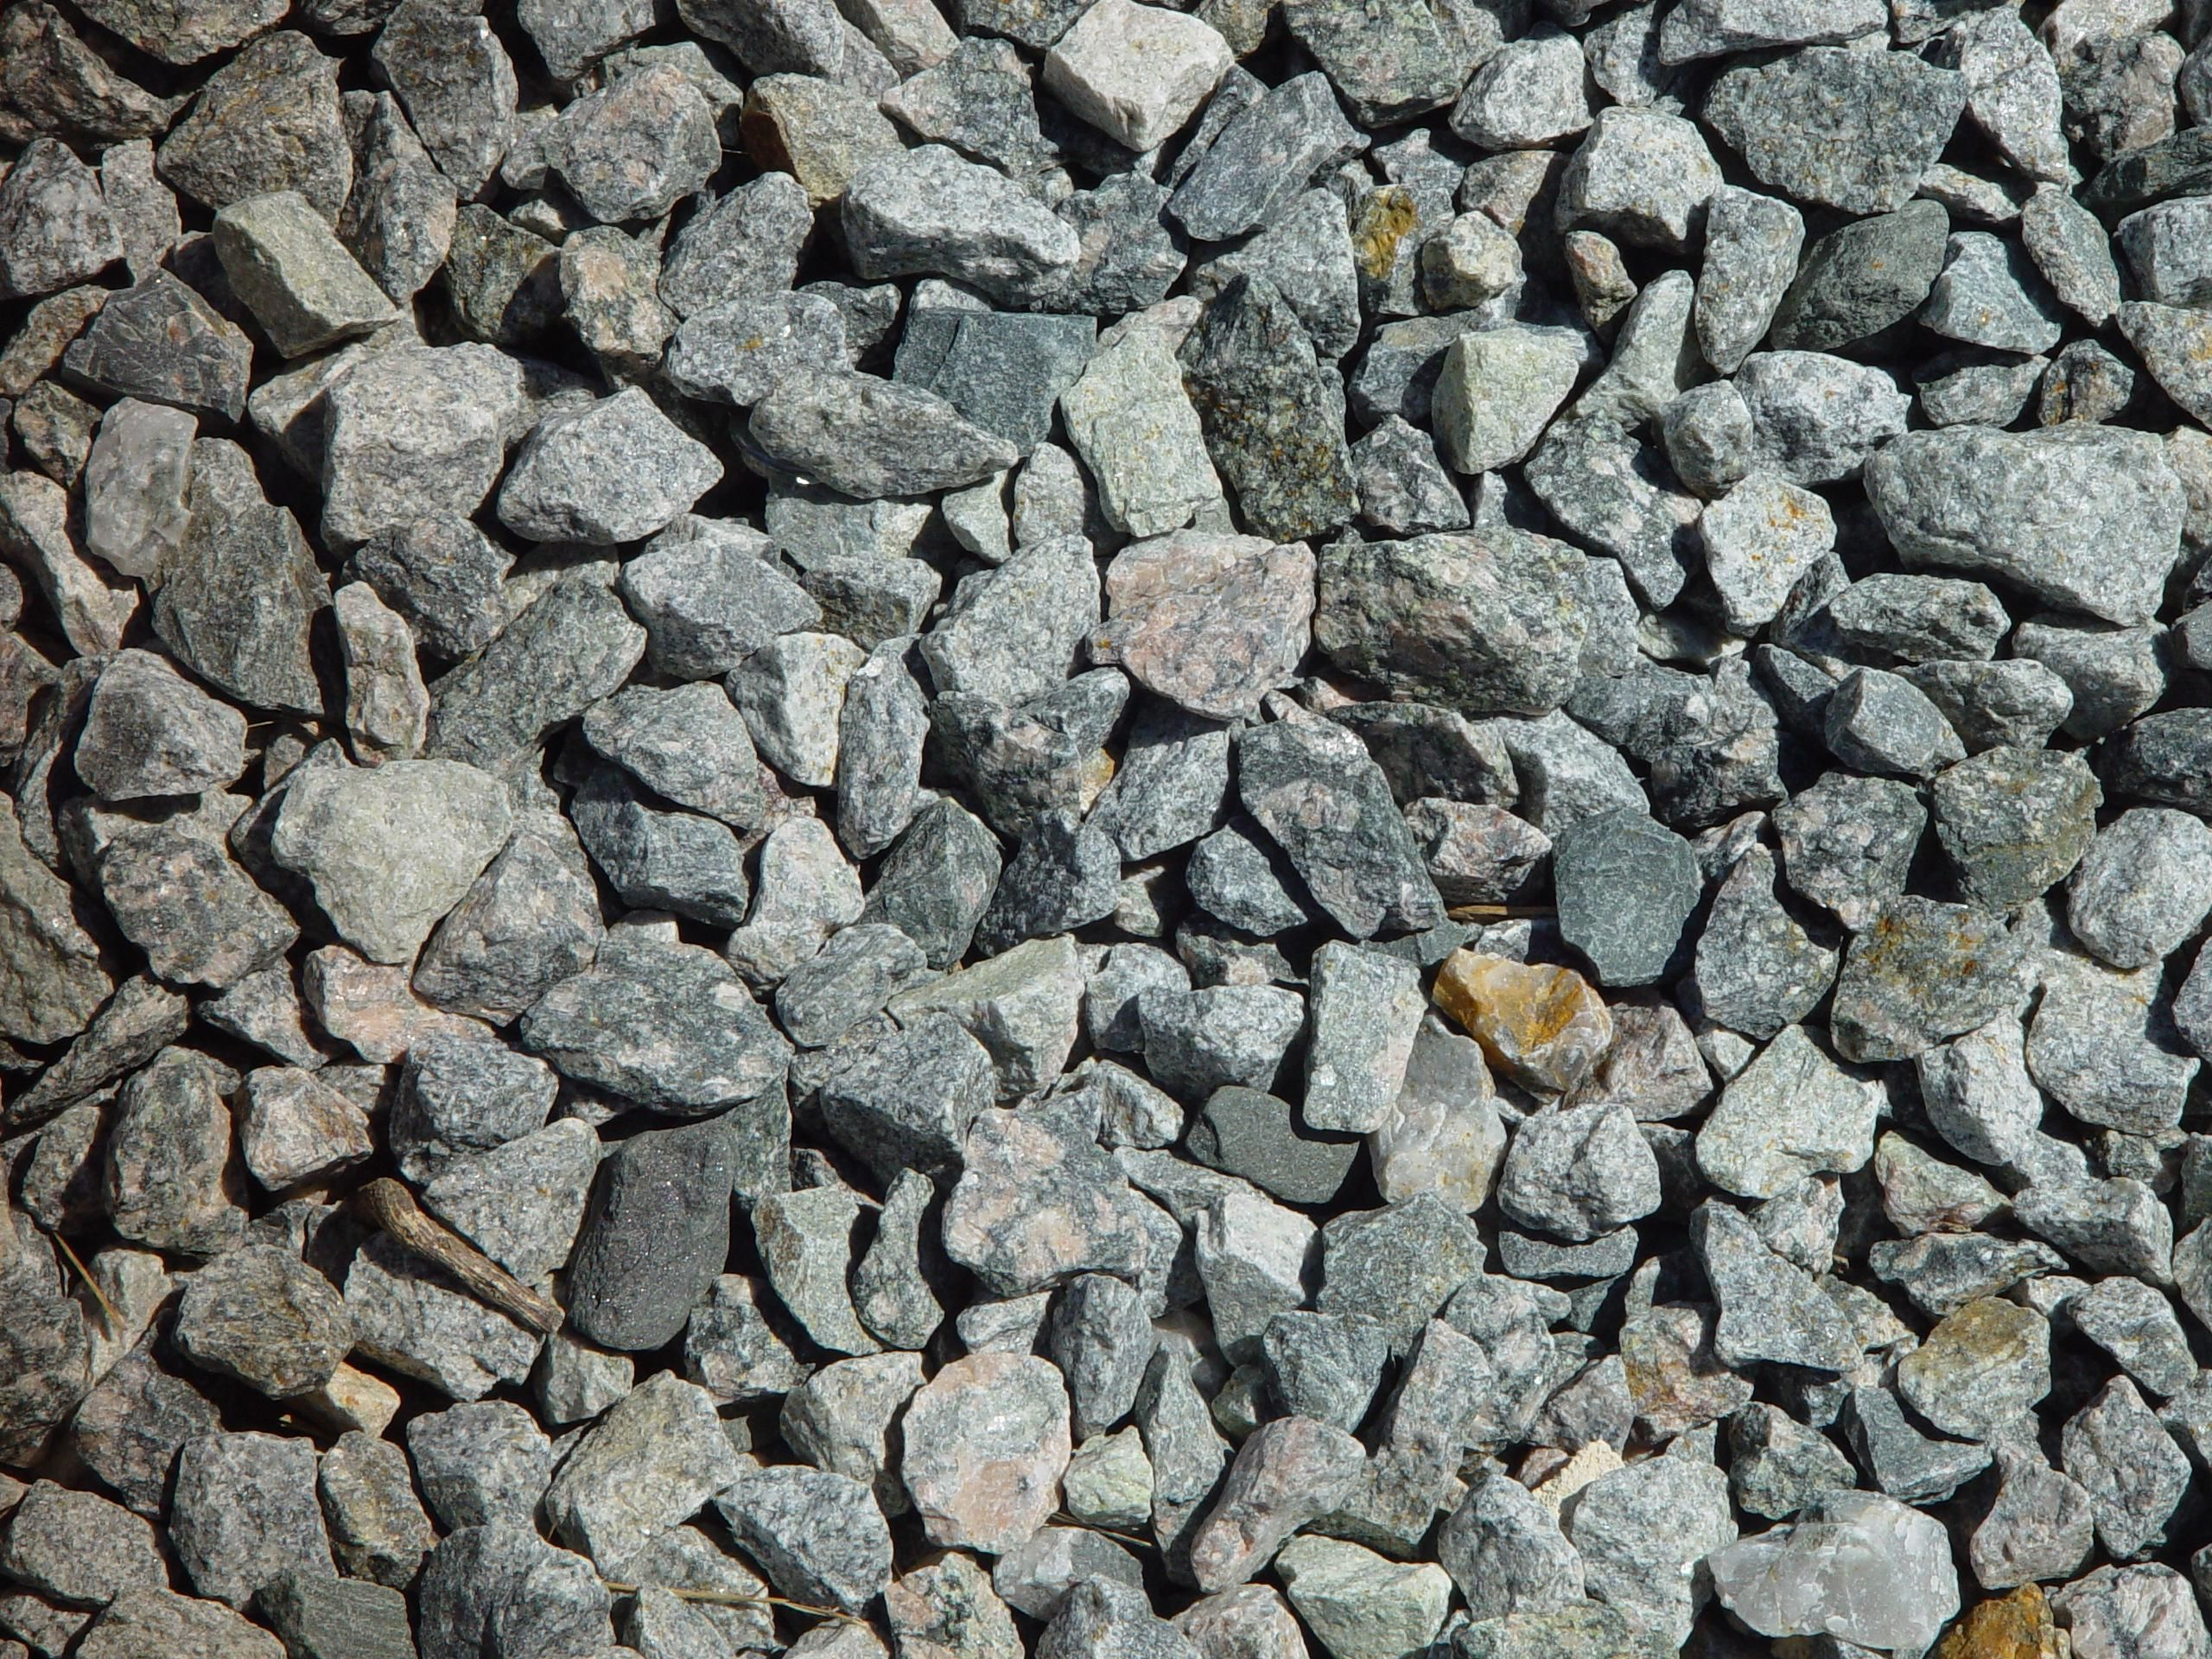
\includegraphics[width=.50\columnwidth]{images/133gravel}
\caption[Gravel]{Gravel.}
\label{fig:133gravel}
\end{figure}
\begin{figure}[!htb]
\centering
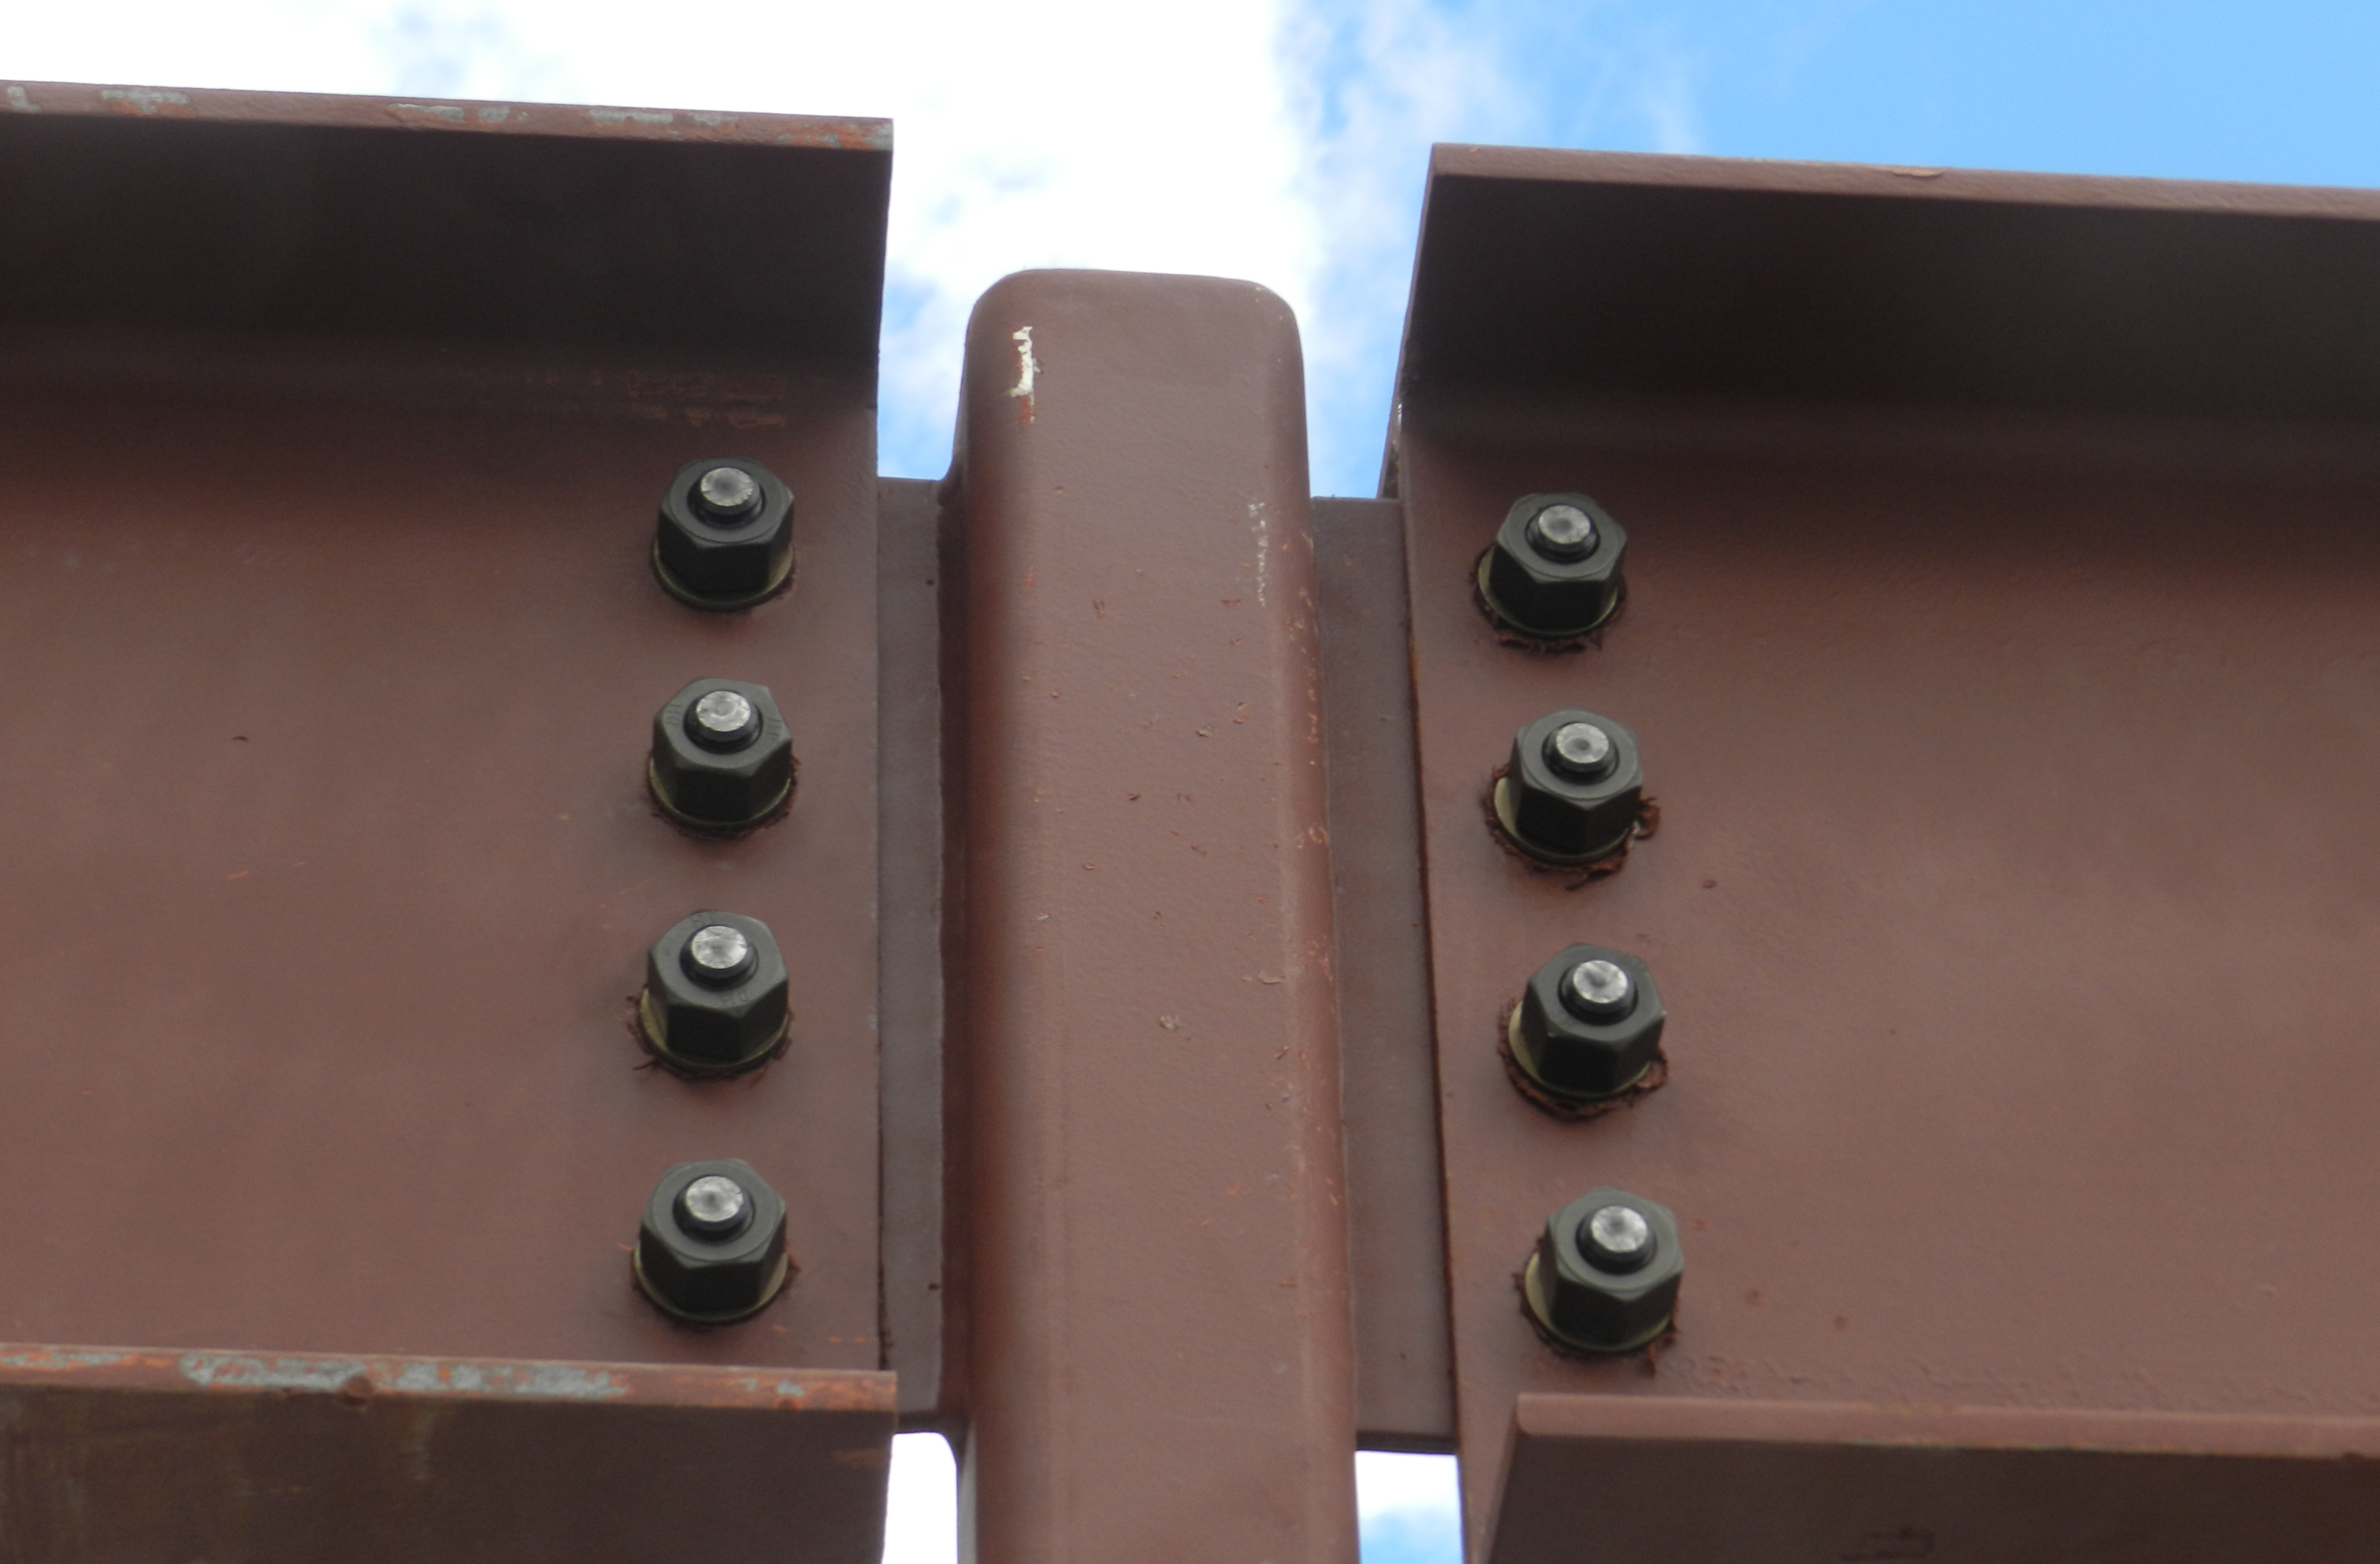
\includegraphics[width=.50\columnwidth]{images/050steel}
\caption[Steel]{Steel.}
\label{fig:050steel}
\end{figure}
In fact, gravels, Fig. \ref{fig:054bsgmaterials}, or granular particles in
general, are far from being a well-defined and easy to characterize material,
like for instance a steel beam, Fig.
\ref{fig:050steel}. For continuous materials simulation
parameters are readily available.
In case of a pile of particles the sum of discrete particle properties determines the pile's macroscopic behavior 
(e.g. angle of repose).
In discrete particle simulations particle based parameters (e.g. contact parameters) determine the macroscopic behavior 
of the ensemble.
Unfortunately, particles are not uniform and particle based simulation
parameters are difficult to obtain, and also depends on the numerical shape
(polyhedral, multi-spheres, and simple spheres).
A set of experimental and numerical solutions, together with artificial neural
networks, could improve the accuracy and the range of applicability of the
characterization of particles properties, and reduce the computational costs.
The Discrete Element Method requires parameters for the individual contact, but
to characterize every particle is prohibitive.
We needed to find average contact parameters that lead to the expected bulk
effect.
We could start with an example of piled particles, more specifically called the
drained angle of repose. This angle of repose, see Fig. \ref{fig:060aor},
characteristic of the bulk macroscopic behaviour of the ensemble, is originated from the microscopic
characteristics of each particle.
\begin{figure}[htbp]
  %\null\hfill
  \subfloat[Silibeads angle of repose.]{
	  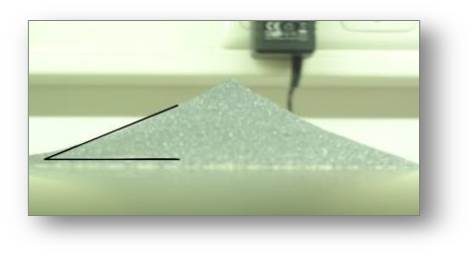
\includegraphics[width=.48\columnwidth]{images/058silibeads}
	  \label{fig:058silibeads}
  }
  \quad
 % \hfill
  \subfloat[Sinter pellets  angle of repose.]{
	  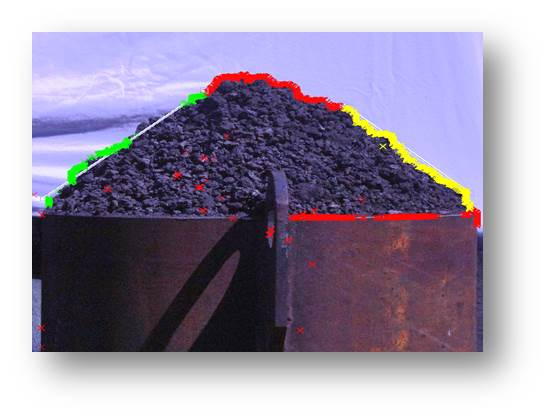
\includegraphics[width=.48\columnwidth]{images/059sinterpellets}
	  \label{fig:059sinterpellets}
  }
 % \hfill\null
  \caption{Angle of repose identification.}
  \label{fig:060aor}
\end{figure}
Once measured the bulk parameter value, through calibration we could obtain the
individual contact parameters:
\begin{enumerate}
\item{we chose initial set of parameters;}
\item{we performed a DEM simulation;}
\item{we compared macroscopic DEM simulation results with experiments;}
\item{if they matched we ended the loop, otherwise we started again from 1 with
new parameters.}
\end{enumerate}
By our calibration procedure we could obtain valid sets of particle based
simulation parameters in a very time consuming way, because in each control loop
we would have to perform a complete \acs{DEM} simulation.
A feasibility study
\info{cite my first paper}
required a grand total of
9.900 days on a 32 core machine. 
But it is not necessary to evaluate a huge number of parameter sets,
rather we should try to evaluate the \textit{sensitivity} 
of the macroscopic bulk behavior with respect to individual particle based parameters.
This could be realized efficiently by artificial neural networks, see Fig.
\ref{fig:048neuron0}. 
After the original work of \citet{RefWorks:189} we know that the human brain is
composed of neurons and their connections. 
They receive inputs from receptive
nerves and together elaborate an output response (e.g., to remove the hand from
a hot surface).
\begin{figure}[!htb]
\centering
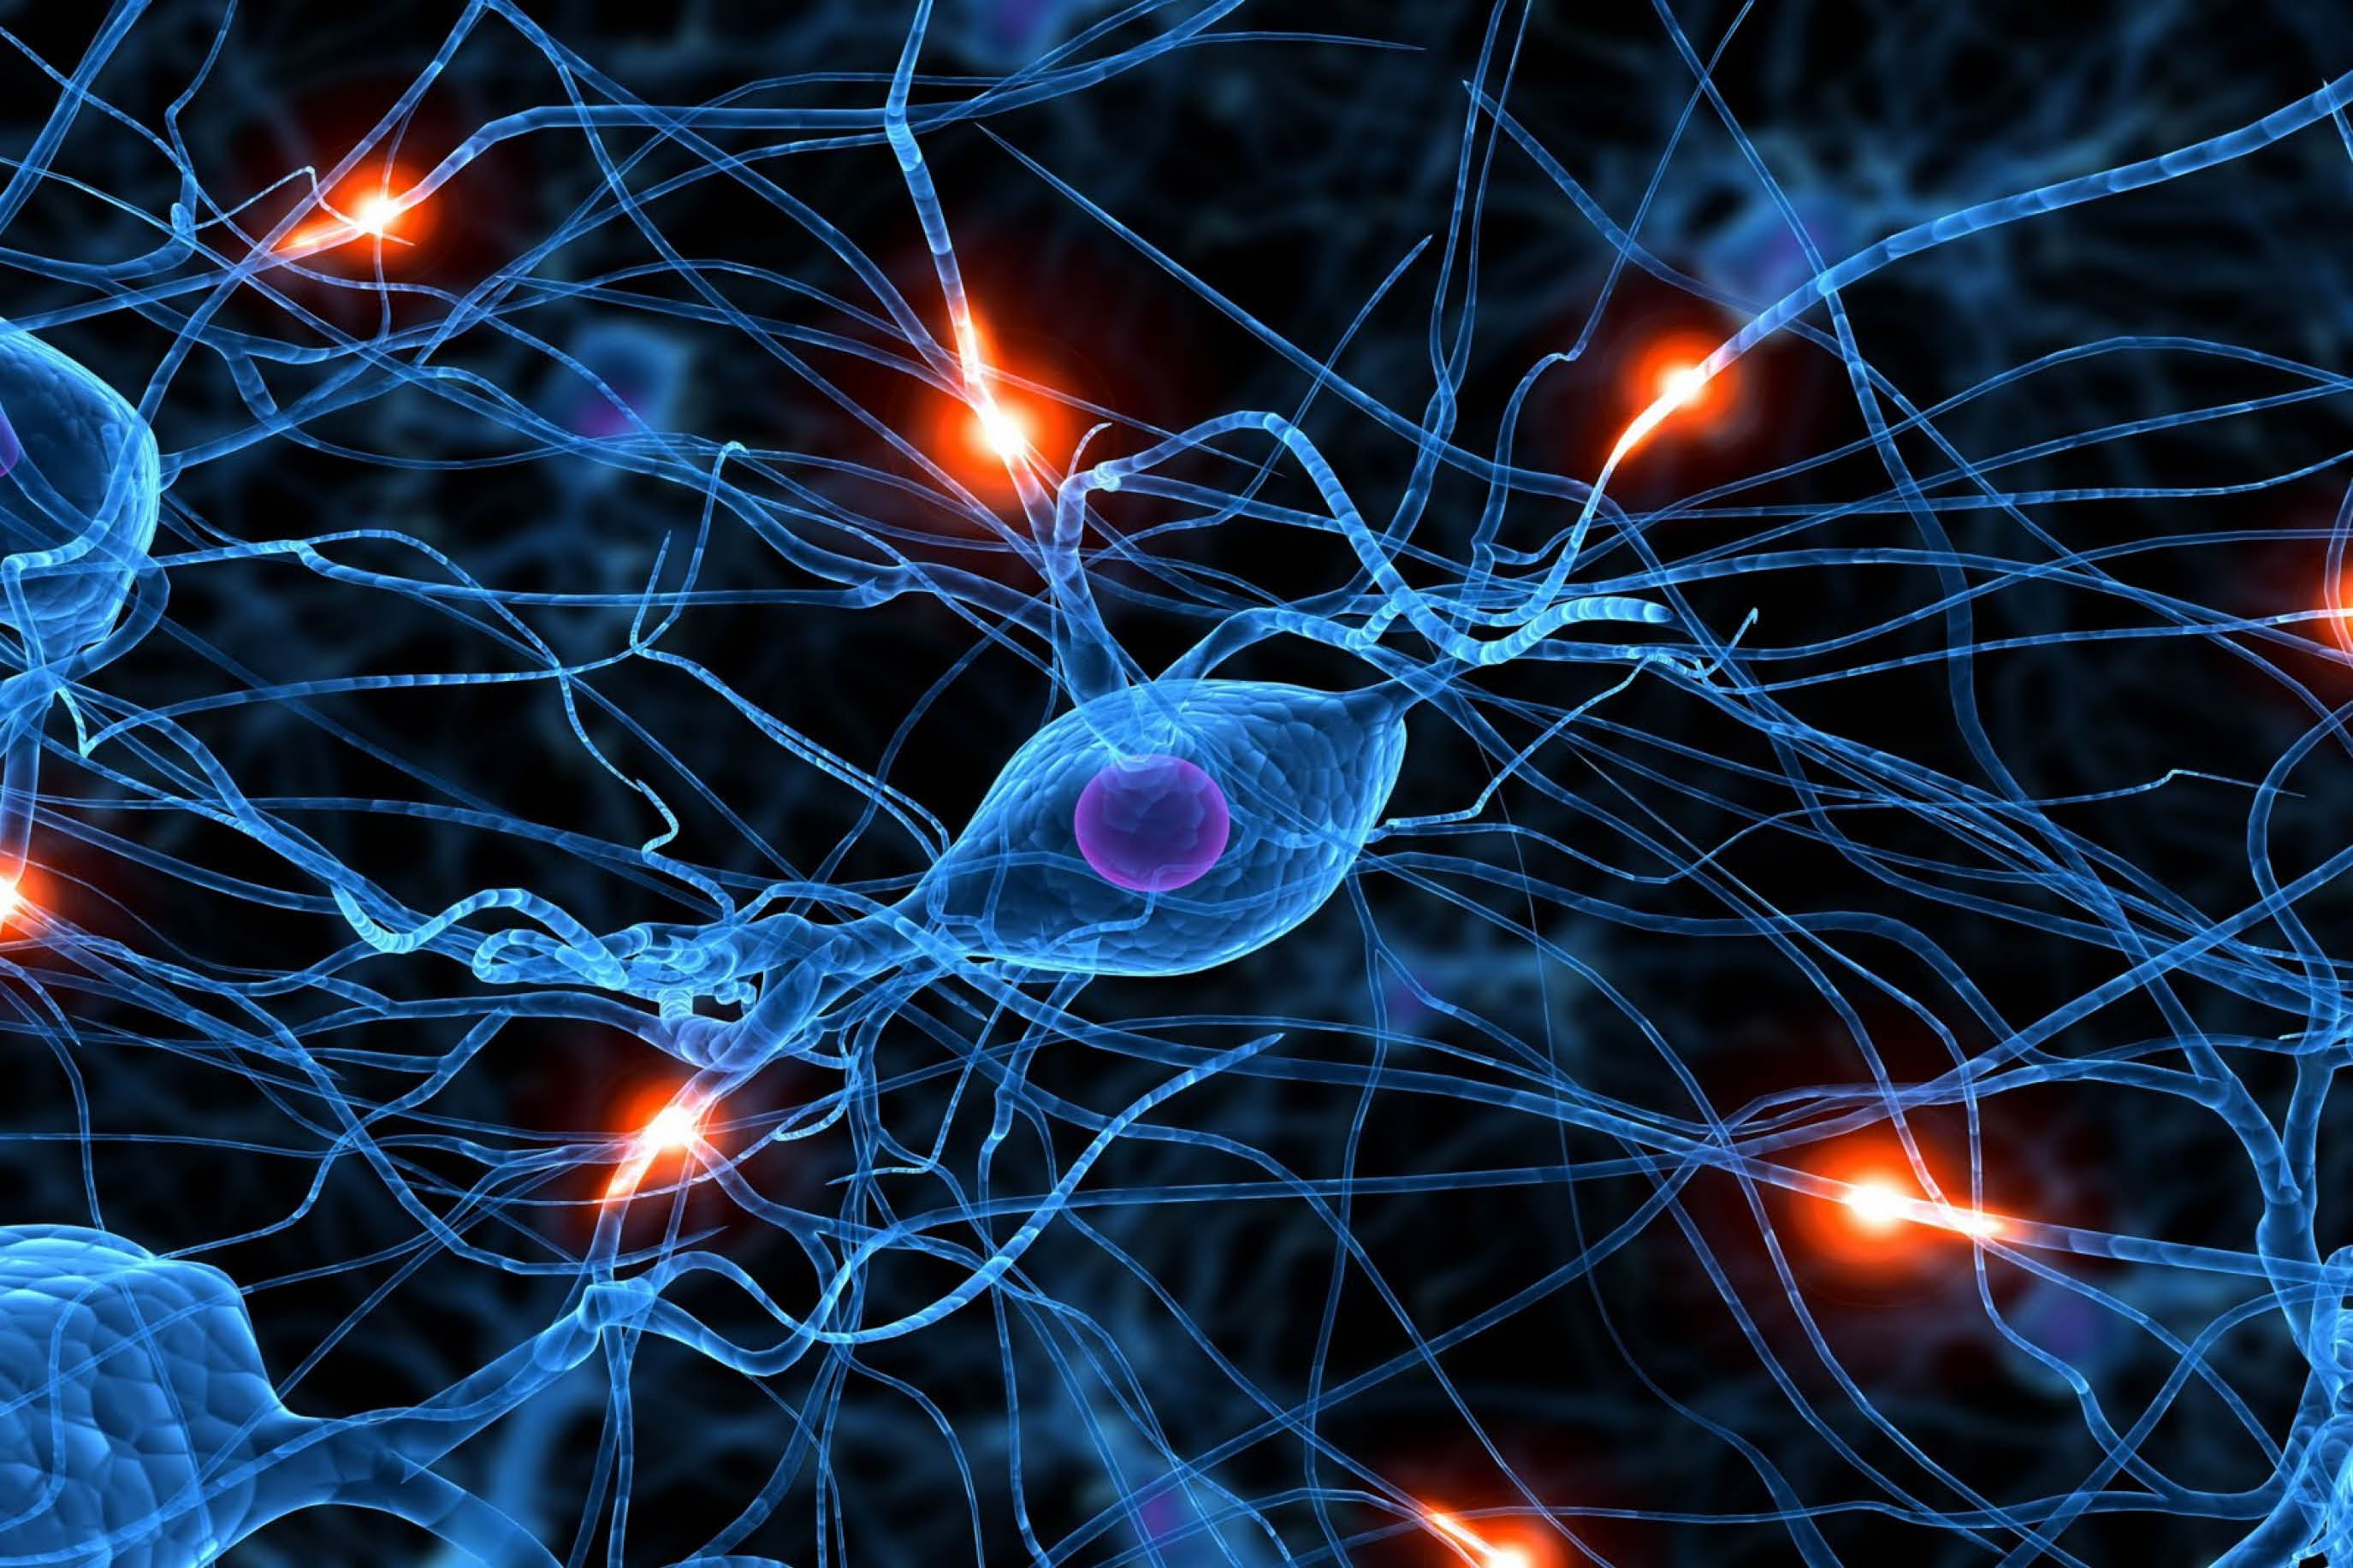
\includegraphics[width=.50\columnwidth]{images/048neuron0}
\caption[Biological inspiration]{Biological inspiration for the Artificial
Neural Networks: a human neuron with the incoming electric signals
\cite{RefWorks:158}.}
\label{fig:048neuron0}
\end{figure}
Similarly, in the artificial neural network we trained a series of neurons.
They had
as inputs particle based parameters and as output the corresponding \acs{DEM}
simulation results.
With both data the network was trained (i.e. individual neurons are
weighted).
Later, the trained neural network could be used to predict additional valid sets
of particle based simulation parameters.

\begin{enumerate}
\item{We trained a neural network by approximately 500 dedicated DEM simulations
(time consuming);}
\item{we predicted another 6.250.000 combinations by the neural network (very
fast);}
\item{we checked if predictions of neural network are correct (by comparing with
experimental  values).}
\end{enumerate}

Typically, less than 1\% of the predicted parameter sets lead to correct
macroscopic results (i.e. 6.000 to 60.000 valid parameter sets).
By this assessment of particle based simulation parameters we obtained valuable
information about the dependence of bulk solid behavior on individual particle properties.
First we could determine the validity range, mean and variance band of each
input parameter. Next we could determine a probability density function for each
input parameter. Then, we could investigate mutual dependencies.
This calibration procedure was universal in a sense that the same artificial
neural network could be harnessed for different macroscopic bulk behaviors.
This effort was really necessary because the predictive capability of any
\acs{DEM} simulation strongly depends on the validity of the particle 
based simulation parameters.\\
Once we had reliable \acs{DEM} parameters, we could use them for large scale \acs{DEM}
simulations:
\begin{itemize}
\item{a sinter chute segregator;}
\item{the raceway zone of a blast furnace.}
\end{itemize}